\section{Evaluation}
The evaluation of the clustering algorithms was performed on a Intel i7 1.70 GHz processor (12th gen.) with 16 GB of RAM running Windows 11.

The evaluation of MAFIA was performed using \textit{GPUMAFIA} \cite{gpumafia}, which was installed on a virtual machine(VM) running Ubuntu 24.04.1 LTS using VirtualBox. The VM was configured with 4 CPUs and 4 GB of RAM. In contrast, CLIQUE and SUBCLU were evaluated on the main machine (host) using ELKI \cite{elki}. Thus, one should be careful to compare the results of MAFIA with those of CLIQUE and SUBCLU, as the execution environment may affect the results, however, their growth rate can be compared.

A range of input parameters (mainly, $\alpha$, $\beta$ and the maximum number of windows) was tested. The best paramters used for each of the tests can be found in the evaluation project in the GitHub repository: \url{https://github.com/henrikdchristensen/SDU-Data-Mining-Exam}. Here, also additional tests as well as detailed descriptions of how to generate the data sets and how to install and use GPUMAFIA.

\subsection{Data set generation}
The aim for synthetic data generation was to be able to produce similar data sets as discussed in \cite{mafia}. Using \textit{MDCGen} it was possible to create large high-dimensional axis-parallel clustered data sets. Here, for example, the number of dimensions, number of clusters, number of data points and percentage of noise can be specified. Furthermore, it was possible to determine for each cluster which of the attributes that are noise, in which we select values at random from a uniform distribution over the entire range of the attribute. Also, all dimensions ranges from 0 to 1.

However, to see the difference between CLIQUE and MAFIA against the SUBCLU algorithm, a data set containing a Bezier-shaped cluster was created using \textit{Artificial Cluster} (AC). Also, a self-populated data set containing a plus-shaped cluster was created as discussed in \cite{mafia}.

\subsection{Experimental Results}

\subsubsection{Scalability with Data Set Size}
The first test was to evaluate the scalability of the algorithms with increasing data set size. The data set used contains 20 dimensions with 5 clusters in 5 different subspaces with 10\% noise records. The data set size ranges from 10k to 15mio records. However, only MAFIA was able to handle the full amount of data. CLIQUE could handle up to 7mio records, while SUBCLU was only able to handle up to 200k records. The results clearly shows that MAFIA is the most scalable algorithm of the three. The results can be seen in Figure \ref{fig:dataset_size_vs_runtime}.
\begin{figure}
    \centering
    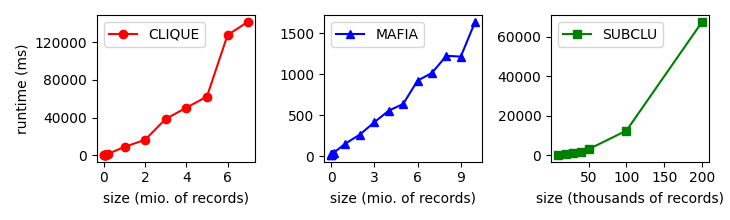
\includegraphics[scale=0.5]{figures/dataset_size_vs_runtime.png}
    \caption{Scalability with increasing data set size.}
    \label{fig:dataset_size_vs_runtime}
\end{figure}

\subsubsection{Clustering Accuracy}
Many different data sets were generated to test the clustering accuracy of the algorithms.

The first data set were a 2-dimensional data set containing a single cluster formed as a plus, as discussed in \cite{mafia}. MAFIA, was able to detect the 2-dimensional cluster almost completly, however, it comes with a cost, as it also will report some lower-dimensional clusters as well. In contrast, CLIQUE was only able to partly detect the cluster and reports two overlapping clusters. The results can be seen in Figure \ref{fig:accuracy_plus}.
\begin{figure}
    \centering
    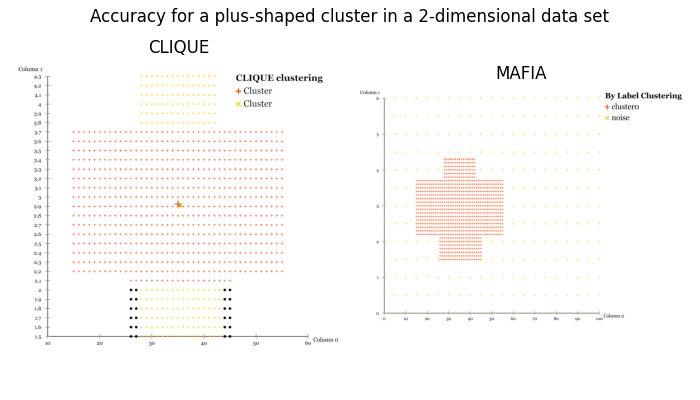
\includegraphics[scale=0.32]{figures/accuracy_plus.png}
    \caption{Plus-shaped cluster.}
    \label{fig:accuracy_plus}
\end{figure}

The second data set contains 10 dimensions with contains 2 clusters embedded in a different 4 dimensional subspace. 10\% of the data was added as noise records. The results can be seen in Figure \ref{fig:accuracy_2clusters}. Here, MAFIA was able to detect the clusters without any additional lower-dimensional clusters. In contrast, CLIQUE reports some overlapping clusters and some of the noise records as clusters. SUBCLU detects also the two clusters, but reports many lower-dimensional clusters and noise records as clusters as well.
\begin{figure}
    \centering
    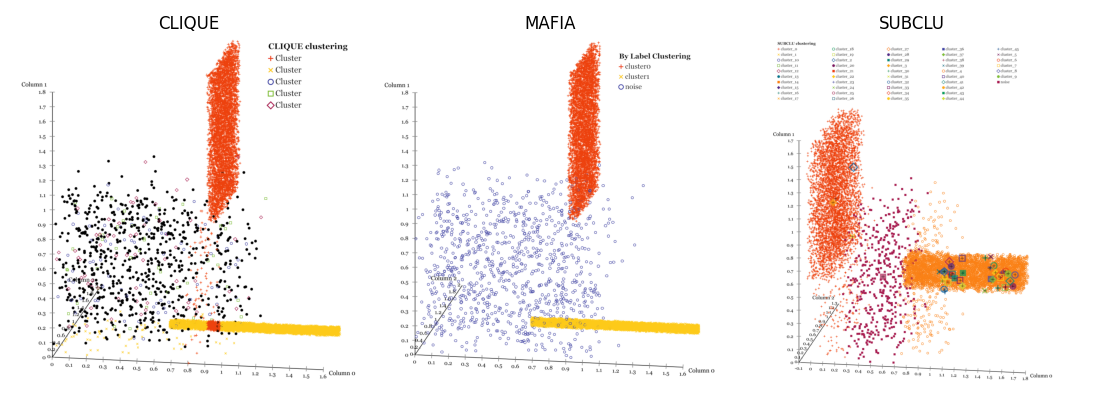
\includegraphics[scale=0.38]{figures/accuracy_2clusters.png}
    \caption{Clusters in different subspaces.}
    \label{fig:accuracy_2clusters}
\end{figure}

The third data set were a 2-dimensional data set containing a single cluster formed as a Bezier curve. Here SUBCLU outperforms the two other algorithms as can be seen in Figure \ref{fig:accuracy_bezier}. MAFIA and CLIQUE only partly detects the cluster. The performance of SUBCLU clearly shows it use of DBSCAN that it runs for separably for each dimension.
\begin{figure}
    \centering
    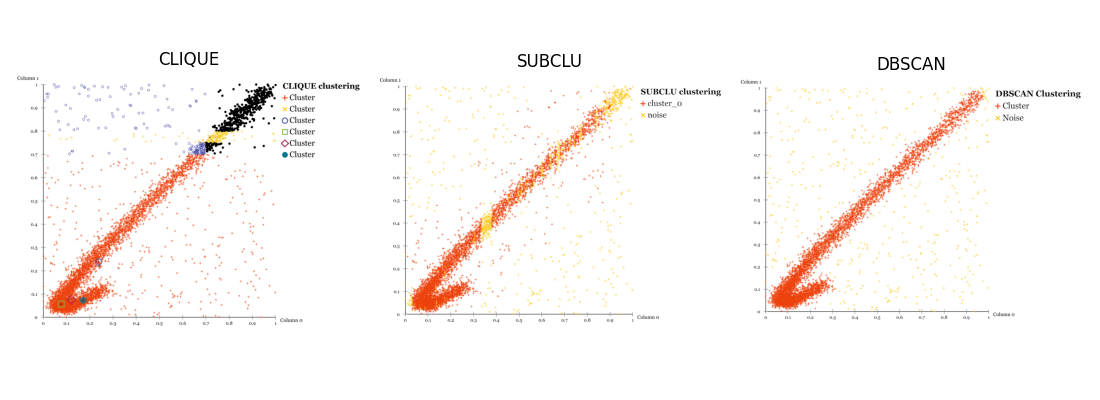
\includegraphics[scale=0.4]{figures/accuracy_bezier.png}
    \caption{Bezier-shaped cluster.}
    \label{fig:accuracy_bezier}
\end{figure}

\subsubsection{Scalability with Data Dimensionality and Cluster Dimensionality}
Figure \ref{fig:data_dimensionality_vs_runtime} shows the scalability of the CLIQUE and MAFIA with increasing data set dimensionality. The data set contains 1 mio. records with 3 clusters in 5 different subspaces and 10\% noise records. The data set dimensionality ranges from 10 to 100 dimensions. The results clearly shows that MAFIA is the most scalable algorithm.
\begin{figure}
    \centering
    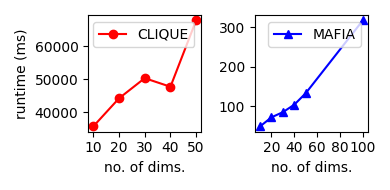
\includegraphics[scale=0.5]{figures/data_dimensionality_vs_runtime.png}
    \caption{Scalability with increasing data set dimensionality.}
    \label{fig:data_dimensionality_vs_runtime}
\end{figure}

Figure \ref{fig:cluster_dimensionality_vs_runtime} shows the scalability of the CLIQUE and MAFIA with increasing cluster dimensionality. The data set contains 500k records with one single cluster. The cluster was embeeded in increasing number of dimensions starting from 10 to 100 dimensions. 10\% of the records was added as noise. The data set contains in total 20 dimensions. The results clearly shows that MAFIA is the most scalable algorithm.
\begin{figure}
    \centering
    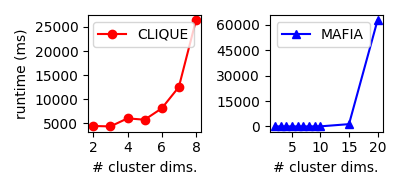
\includegraphics[scale=0.5]{figures/cluster_dimensionality_vs_runtime.png}
    \caption{Scalability with increasing cluster dimensionality.}
    \label{fig:cluster_dimensionality_vs_runtime}
\end{figure}

The results reported for SUBCLU \cite{subclu} were also tried to be replicated, however, similar results were not achieved.

\subsection{Sensitive analysis for MAFIA}
To see how sensitive MAFIA is to the input parameters, we tests its sensitivity to the $\alpha$ parameter. The data set used was a 20-dimensional data set with 1mio data points, where 10\% was outliers. In this test, $\beta$ was fixed, and $\alpha$ was ranging from 0.8 to 5.2 in step size of 0.4. The results can be seen in Figure \ref{fig:sensitivity_alpha}. From the results one could draw the conclusion that MAFIA is not very sensitive to the $\alpha$ parameter. However, from the tests conducted throughout the evaluation, many different values $\alpha$ was used to detect the right clusters. So the alpha parameter is somehow nested to the type of data set. The same goes for the $\beta$ and the maximum number of windows.
\begin{figure}
    \centering
    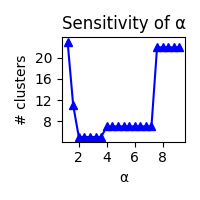
\includegraphics[scale=0.6]{figures/sensitivity_alpha.png}
    \caption{Sensitive analysis for MAFIA.}
    \label{fig:sensitivity_alpha}
\end{figure}

\subsubsection{Real Data Sets}
Two real-world data sets are used to evaluate the algorithms in a more realistic setting. Small data sets were selected for both performance and visualization reasons. Both data sets were normalized such that each attribute was in the range [0, 1].

The first data set is well-known \textit{Iris} data set \cite{iris}, which contains 150 records of 3 different iris types (e.g. Setosa, Versicolor, Virginica). The data set contains 4 features (sepal length, sepal width, petal length and petal width). All three algorithms produced some meaningful clusters, however, as can be seen in Figure \ref{fig:real_world_iris}, SUBCLU seems to be the best of the three.
\begin{figure}
    \centering
    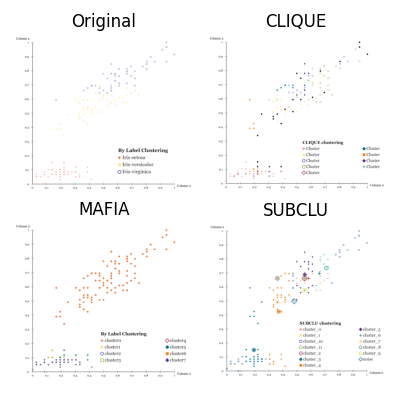
\includegraphics[scale=0.5]{figures/real_world_iris.png}
    \caption{Iris data set.}
    \label{fig:real_world_iris}
\end{figure}

The second data set is the \textit{Date Fruit} data set \cite{date-fruit}, which contains 898 records of 7 different date fruit types (e.g. Barhee, Deglet Nour, Sukkary, Rotab). These were obtained via a computer vision, where 34 features (e.g shape and color) was extracted. Only SUBCLU were able to produce meaningful results, see Figure \ref{fig:real_world_date_fruit}.
\begin{figure}
    \centering
    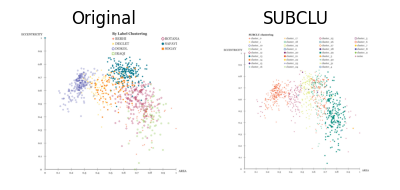
\includegraphics[scale=0.5]{figures/real_world_date_fruit.png}
    \caption{Date Fruit data set.}
    \label{fig:real_world_date_fruit}
\end{figure}